\documentclass{article}

\usepackage{blindtext}
\usepackage[
	backend = biber,
	style = bwl-FU,
	url = false,
	doi = false,
	eprint = false
]{biblatex}
\addbibresource{Biblio.bib}
\usepackage{graphicx}
\usepackage{threeparttable}


\begin{document}

\title{This is a title}
\author{Marco Barcellos\thanks{I'd like to thank my cats for their support.} \\ \normalsize{University of Zürich}}
\date{\today}
\maketitle
\begin{abstract}
This abstract is irrelevant. Don't listen to it.
\end{abstract}
\section{Introduction}
\Blindtext
For further information, refer to \cite{corona} and \cite{Tail}.
\par

\emph{Figure \ref{figure1} contains an image illustrating a cat. Thereafter comes table \ref{table:1}, containing names of beers named after cats.}
\newpage

	\begin{figure}[htb]\center 
		\begin{tabular}{c}
			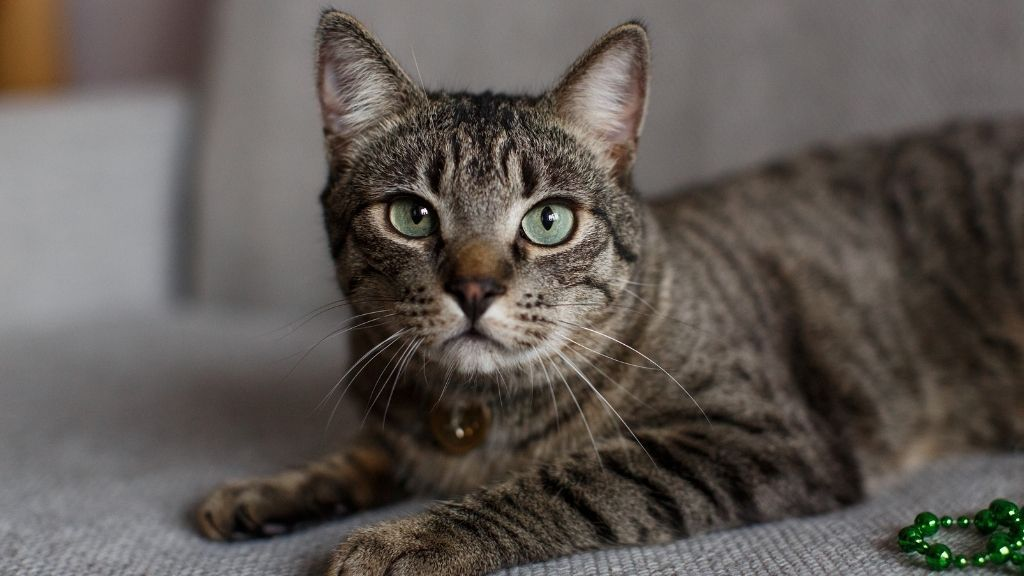
\includegraphics[width = 10cm]{cat.jpg}
		\end{tabular}
		\caption{\footnotesize This is a cat}
		\label{figure1}
	\end{figure}


\begin{table}[h!]
\center
\begin{tabular}{ |c||c|r|l|  }
 \hline
 \multicolumn{4}{|c|}{Cat title} \\
 \hline
 Cat Name & Country of Origin &Type of Cat&Catness\\
 \hline
 Krombacher   & Germany    & Pils &   6/10\\
 Oettinger&   Germany  & Export   &10/10\\
 Feldschlösschen &Switzerland & Lager &  5/10\\
 Heineken    &Netherlands & Lager &  5/10\\
 Pilsner Urquell&   Czech Republic  & Pils & 7/10\\
 Arany Àszok& Hungary  & Lager   & 2/10\\
 Dreher& Hungary  & Pils & 5/10\\
 \hline
 \end{tabular}
 \caption{This is a cat table}
 \label{table:1}
\end{table}

\newpage

\printbibliography

\end{document}